\section{Invertibility and Isomorphisms} \label{sec 2.4}

We see in this section (\THM{2.17}) that the \emph{inverse} of a \LTRAN{} is also linear(if it exists).
This result greatly aids us in the study of \emph{inverses of matrices}.
As one might expect from \SEC{2.3}, the inverse of the left-multiplication transformation \(\LMTRAN_A\) (when it exists) can be used to determine properties of the inverse of the matrix \(A\).

In the remainder of this section, we apply many of the results about invertibility to the concept of \emph{isomorphism} (\DEF{2.14}).
We will see that \emph{finite}-dimensional vector spaces (over \(F\)) of \emph{equal dimension} may be \emph{identified} (by \(F^n)\).
These ideas will be made precise shortly.

\begin{definition} \label{def 2.12}
Let \(V\) and \(W\) be vector spaces, and let \(\T : V \to W\) be linear.

\BLUE{(1)} A function \(\U: W \to V\) is said to be an \textbf{inverse} of \(\T\) if \(\T\U = \ITRANW\) \textbf{and} \(\U\T = \ITRANV\).

\BLUE{(2)} If \(\T\) has an inverse, then \(\T\) is said to be \textbf{invertible}.

\BLUE{(3)} As noted in Appendix B, if \(\T\) is invertible, then the inverse of \(\T\) is \textbf{unique} and is denoted by \(\T^{-1}\).
\end{definition}

\begin{additional theorem} \label{athm 2.35}
The following facts hold for \emph{invertible} functions \(\T\) and \(\U\).

\BLUE{(1)} \((\T\U)^{-1} = \U^{-1} \T^{-1}\).

\BLUE{(2)} \((\T^{-1})^{-1} = \T\)
(For \(\T^{-1}\), there exists \(\T\) s.t. \(\T^{-1}\T = \ITRANV\) and \(\T\T^{-1} = \ITRANW\),
hence by definition \(\T\) is the inverse of \(\T^{-1}\), that is, (since \((\T^{-1})^{-1}\) is unique,) \((\T^{-1})^{-1} = \T\));
in particular, \(\T^{-1}\) is invertible.

We often use the fact that a function is invertible if and only if it is both one-to-one and onto.
We can therefore restate \THM{2.5} as follows.

\BLUE{(3)}: Let \(\T : V \to W\) be a \LTRAN{}, where \(V\) and \(W\) are \emph{finite}-dimensional spaces of \emph{equal dimension}.
Then \(\T\) is invertible if and only if \(\rankT = \dim(V)\).
(\(\T\) is invertible iff \(\T\) is one-to-one and onto, iff (by \THM{2.5}(c)) \(\rankT = \dim(V)\).)
\end{additional theorem}

\begin{example} \label{example 2.4.1}
Let \(\T : \mathcal{P}_1(\SET{R}) \to \SET{R}^2\) be the \LTRAN{} defined by \(\T(a + bx) = (a, a + b)\).
The reader can verify directly that \(\T^{-1} : \SET{R}^2 \to \mathcal{P}_1(\SET{R})\) is defined by \(\T^{-1}(c, d) = c + (d - c)x\).
Observe that \(\T^{-1}\) is also linear.
As \THM{2.17} demonstrates, this is true in general.
\end{example}

\begin{theorem} \label{thm 2.17}
Let \(V\) and \(W\) (over common \(F\)) be vector spaces, and let \(\T : V \to W\) be linear and invertible.
Then \(\T^{-1} : W \to V\) is linear.
\end{theorem}

\begin{note}
We do not assume \(V, W\) to be finite-dimensional.
\end{note}

\begin{proof}
Let \(y_1, y_2 \in W\) and \(c \in F\).
Since \(\T\) is onto and one-to-one, there exist \emph{unique} vectors \(x_1\) and \(x_2\) in \(V\) such that \(\T(x_1) = y_1\) and \(\T(x_2) = y_2\) \MAROON{(1)}.
Thus (by definition of inverse function) \(x_1 = \T^{-1}(y_1)\) and \(x_2 = \T^{-1}(y_2)\) \MAROON{(2)}; so

\begin{align*}
    \T^{-1}(cy_1 + y_2) & = \T^{-1}(c\T(x_1) + \T(x_2)) & \text{by \MAROON{(1)}} \\
                        & = \T^{-1}(\T(cx_1 + x_2)) & \text{since \(\T\) is linear} \\
                        & = cx_1 + x_2 & \text{since \(\T^{-1}\T = \ITRANV\)} \\
                        & = c\T^{-1}(y_1) + \T^{-1}(y_2) & \text{by \MAROON{(2)}}
\end{align*}
So by \ATHM{2.1}(b), \(\T^{-1}\) is linear.
\end{proof}

\begin{corollary} \label{corollary 2.17.1}
Let \(\T\) be an invertible \LTRAN{} from \(V\) to \(W\).
Then \(V\) is finite-dimensional if and only if \(W\) is finite-dimensional.
In the case where both dimensions are finite, we have \(\dim(V) = \dim(W)\).
\end{corollary}

\begin{proof}
Suppose that \(V\) is finite-dimensional. Let \(\beta = \{ x_1, x_2, ..., x_n \}\) be a basis for \(V\).
By \THM{2.2}, \(\spann(\T(\beta)) = \RANGET\).
Since \(\T\) is (in particular) onto, \(\RANGET = W\).
So \(W\) can be generated by a finite set \(\T(\beta)\), hence by \THM{1.9} \(W\)'s basis is finite, hence \(W\) is finite-dimensional.

Conversely, if \(W\) is finite-dimensional. Let \(\gamma = \{ y_1, y_2, ..., y_m \}\) be a basis for \(W\).
By \THM{2.2}, \(\spann(\T^{-1}(\gamma)) = \RANGE(\T^{-1})\).
Since \(\T^{-1}\) is (in particular) onto, \(\RANGE(\T^{-1}) = V\).
So \(V\) can be generated by a finite set \(\T^{-1}(\gamma)\), hence by \THM{1.9} \(V\)'s basis is finite, hence \(V\) is finite-dimensional.

Now suppose that \(V\) and \(W\) are finite-dimensional.
Because \(\T\) is one-to-one and onto, we have
\begin{align*}
    \dim(V) & = \nullityT + \rankT & \text{by dimension theorem, \THM{2.3}} \\
            & = 0 + \rankT & \text{since \(\T\) is one-to-one} \\
            & = 0 + \dim(W) & \text{since \(\T\) is onto} \\
            & = \dim(W).
\end{align*}
\end{proof}

\begin{remark} \label{remark 2.4.1}
It now follows immediately from \THM{2.5} that if \(\T\) is a \LTRAN{} between vector spaces of equal (\emph{finite}) dimension, then \emph{the conditions of being invertible, one-to-one, and onto are all equivalent}.
\end{remark}

We are now ready to define the \emph{inverse} of a matrix.
The reader should note the analogy with the inverse of a \LTRAN{}(\DEF{2.12}).

\begin{definition} \label{def 2.13}
Let \(A\) be an \(n \X n\) matrix.

\BLUE{(1)} Then \(A\) is \textbf{invertible} if there exists an \(n \X n\) matrix \(B\) such that \(AB = I\) \textbf{and} \(BA = I\).
(from the context, \(I\) is in fact \(I_n\), the \(n \X n\) identity matrix.)
\end{definition}

\BLUE{(2)} If \(A\) is invertible, then the matrix \(B\) such that \(AB = BA = I\) \emph{is} unique, since if \(G\) were another such matrix, then
\begin{align*}
    G & = GI & \text{by \THM{2.12}(c)} \\
      & = G(AB) & \text{since \(AB = I\)} \\
      & = (GA)B & \text{by \THM{2.16}, associative} \\
      & = IB & \text{by supposition} \\
      & = B. & \text{by \THM{2.12}(c)}
\end{align*}

\BLUE{(3)} The matrix \(B\) is called the \textbf{inverse} of \(A\) and is denoted by \(A^{-1}\).

\begin{example} \label{example 2.4.2}
Trivial.
\end{example}

In \SEC{3.2}, we will learn a \textbf{technique for computing the inverse of a matrix}.
At this point, we develop a number of results that \emph{relate the inverses of matrices} to the \emph{inverses of \LTRAN{}s}.

\begin{theorem} \label{thm 2.18}
Let \(V\) and \(W\) be finite-dimensional vector spaces with ordered bases \(\beta\) and \(\gamma\), respectively.
Let \(\T : V \to W\) be linear.
Then \(\T\) is invertible(by \DEF{2.12}) \emph{if and only if} \([\T]_{\beta}^{\gamma}\) is invertible(by \DEF{2.13}).
Furthermore, \([\T^{-1}]_{\gamma}^{\beta} = ([\T]_{\beta}^{\gamma})^{-1}\).
\end{theorem}

\begin{note}
The transformation is invertible if and only if its matrix representation is invertible.
And the matrix representation of the inverse of the transformation is equal to the inverse of the matrix representation of the transformation.
\end{note}

\begin{proof} \ 

\(\Longrightarrow\): Suppose that \(\T\) is invertible.
By the \CORO{2.17.1}, we have \(\dim(V) = \dim(W)\).
Let \(n = \dim(V)\), then \([\T]_{\beta}^{\gamma}\) is an \(n \X n\) matrix.
And by \DEF{2.12}, \(\T^{-1} : W \to V\) satisfies \(\T\T^{-1} = \ITRANW\) \MAROON{(1.1)} and \(\T^{-1}\T = \ITRANV\) \MAROON{(1.2)}.

Then we have
\begin{align*}
    I_n & = [\ITRANV]_{\beta} & \text{trivial, or by \EXEC{2.3.1}(d)} \\
        & = [\T^{-1}\T]_{\beta} & \text{by \MAROON{(1.2)}} \\
        & = [\T^{-1}]_{\gamma}^{\beta} [\T]_{\beta}^{\gamma} & \text{by \THM{2.11}}
\end{align*}
Similarly,
\begin{align*}
    I_n & = [\ITRANW]_{\gamma} & \text{trivial, or by \EXEC{2.3.1}(d)} \\
        & = [\T\T^{-1}]_{\gamma} & \text{by \MAROON{(1.1)}} \\
        & = [\T]_{\beta}^{\gamma} [\T^{-1}]_{\gamma}^{\beta} & \text{by \THM{2.11}}
\end{align*}
So we have found a matrix \( \BLUE{[\T^{-1}]_{\gamma}^{\beta}}\) s.t. \([\T]_{\beta}^{\gamma} \BLUE{[\T^{-1}]_{\gamma}^{\beta}} = I_n = \BLUE{[\T^{-1}]_{\gamma}^{\beta}} [\T]_{\beta}^{\gamma}\),
hence by \DEF{2.13}, \([\T]_{\beta}^{\gamma}\) is invertible, and its (unique) inverse is \(\BLUE{[\T^{-1}]_{\gamma}^{\beta}}\);
that is, \(([\T]_{\beta}^{\gamma})^{-1} = \BLUE{[\T^{-1}]_{\gamma}^{\beta}}\).

\(\Longleftarrow\): Now suppose \(A = [\T]_{\beta}^{\gamma}\) \MAROON{(2.1)} is invertible.
Then by \DEF{2.13} there exists \(B\) s.t. \(AB = BA = I_n\) \MAROON{(2.2)}.

Now we first just label \(\gamma = \{ w_1, w_2, ... w_n \}\) and \(\beta = \{ v_1, v_2, ..., v_n \}\).
Then by \THM{2.6}, we can find a unique \LTRAN{} \(\U : W \to V\) such that it satisfies
\[
    \U(w_j) = \sum_{i = 1}^n B_{ij} v_{i} \text{ for \(j = 1, 2, ..., n\)}
\]
In particular, (by \DEF{2.6},) \([\U]_{\gamma}^{\beta} = B\) \MAROON{(2.3)}.
Finally we have to show \(\U\) is the inverse of \(\T\) (by \DEF{2.12}) by showing \(\U\T = \ITRANV\) and \(\T\U = \ITRANW\).
But observe that
\begin{align*}
    [\U\T]_{\beta} & = [\U]_{\gamma}^{\beta} [\T]_{\beta}^{\gamma} & \text{by \THM{2.11}} \\
                   & = BA & \text{by \MAROON{(2.1), (2.3)}} \\
                   & = I_n & \text{by \MAROON{(2.2)}} \\
                   & = [\ITRANV]_{\beta}, & \text{trivial, or by \EXEC{2.3.1}(d)}
\end{align*}
hence (by \RMK{2.2.2}) \(\U\T = \ITRANV\).
Similarly,
\begin{align*}
    [\T\U]_{\gamma} & = [\T]_{\beta}^{\gamma} [\U]_{\gamma}^{\beta} & \text{by \THM{2.11}} \\
                   & = AB & \text{by \MAROON{(2.3), (2.1)}} \\
                   & = I_n & \text{by \MAROON{(2.2)}} \\
                   & = [\ITRANW]_{\gamma}, & \text{trivial, or by \EXEC{2.3.1}(d)}
\end{align*}
hence (by \RMK{2.2.2}) \(\T\U = \ITRANW\).

So we have shown \(\U\T = \ITRANV\) and \(\T\U = \ITRANW\), so by \DEF{2.12} \(\T\) is invertible, as desired.
\end{proof}

\begin{example} \label{example 2.4.3}
Let \(\beta\) and \(\gamma\) be the standard ordered bases of \(\mathcal{P}_1(\SET{R})\) and \(\SET{R}^2\), respectively.
For \(\T\) as in \EXAMPLE{2.4.1}, we have
\[
    [\T]_{\beta}^{\gamma} = \begin{pmatrix} 1 & 0 \\ 1 & 1 \end{pmatrix}
    \text{ and }
    [\T^{-1}]_{\gamma}^{\beta} = \begin{pmatrix} 1 & 0 \\ -1 & 1 \end{pmatrix}.
\]
It can be verified by matrix multiplication that each matrix is the inverse of the other.
\end{example}

\begin{corollary} \label{corollary 2.18.1}
Let \(V\) be a \emph{finite}-dimensional vector space with an ordered basis \(\beta\), and let \(\T : V \to V\) be linear.
Then \(\T\) is invertible if and only if \([\T]_\beta\)
is invertible.
Furthermore, \([\T^{-1}]_{\beta} = ([\T]_{\beta})^{-1}\).
\end{corollary}

\begin{proof}
This is just a special case of \THM{2.18} where \(W = V\) and \(\gamma = \beta\).
\end{proof}

\begin{corollary} \label{corollary 2.18.2}
Let \(A\) be an \(n \X n\) matrix.
Then \(A\) is invertible if and only if \(\LMTRAN_A\) is invertible. Furthermore, \((\LMTRAN_A)^{-1} = \LMTRAN_{A^{-1}}\).
\end{corollary}

\begin{proof}
Let \(\beta\) be the standard ordered basis of \(F^n\).
(We need \(\beta\) because \(\LMTRAN_A\) is from \(F^n\) to \(F^n\).)
Then in particular by \CORO{2.18.1}, \([\LMTRAN_A]_{\beta}\) is invertible if and only if \(\LMTRAN_A\) is invertible.
But by \THM{2.15}(a), \([\LMTRAN_A]_{\beta} = A\).
So we have \(A\) is invertible if and only if \(\LMTRAN_A\) is invertible.

And in particular, if \(A\) is invertible, then
\begin{align*}
    \mathrm{I}_{F^n} & = \LMTRAN_{I_n} & \text{by \THM{2.15}(f)} \\
                     & = \LMTRAN_{A A^{-1}} & \text{since \(A\) is invertible} \\
                     & = \LMTRAN_A \LMTRAN_{A^{-1}} & \text{by \THM{2.15}(e)},
\end{align*}
similarly,
\begin{align*}
    \mathrm{I}_{F^n} & = \LMTRAN_{I_n} & \text{by \THM{2.15}(f)} \\
                     & = \LMTRAN_{A^{-1} A} & \text{since \(A\) is invertible} \\
                     & = \LMTRAN_{A^{-1}} \LMTRAN_A & \text{by \THM{2.15}(e)}.
\end{align*}
By \DEF{2.12}, the (unique) inverse of \(\LMTRAN_A\) is \(\LMTRAN_{A^{-1}}\).
That is, \((\LMTRAN_A)^{-1} = \LMTRAN_{A^{-1}}\).
\end{proof}

\begin{remark} \label{remark 2.4.2}
The notion of invertibility may be used to formalize what may already have been observed by the reader, that is,
that certain vector spaces \emph{strongly resemble} one another \emph{except for the \textbf{form}} of their vectors.
For example, in the case of \(M_{2 \X 2}(F)\) and \(F^4\), if we associate each matrix
\[
    \begin{pmatrix} a & b \\ c & d \end{pmatrix}
\]
to the \(4\)-tuple \((a, b, c, d)\), we see that \textbf{sums and scalar products associate in a similar manner};
that is, \emph{in terms of the vector space structure}, these two
vector spaces may be considered \textbf{identical or isomorphic}.
\end{remark}

\begin{definition} \label{def 2.14}
Let \(V\) and \(W\) be vector spaces.

\BLUE{(1)} We say that \(V\) is \textbf{isomorphic} to \(W\) if there exists a \emph{linear} transformation \(\T : V \to W\) that is \emph{invertible}.

\BLUE{(2)} Such a \LTRAN{} is called an \textbf{isomorphism} from \(V\) onto \(W\).
\end{definition}

\begin{remark} \label{remark 2.4.3}
We leave as an exercise (see \EXEC{2.4.13}) "is isomorphic to" is an \textbf{equivalence relation}.
So we need only say that ``\(V\) and \(W\) are isomorphic''.
\end{remark}

\begin{example} \label{example 2.4.4}
Define \(\T : F^2 \to \mathcal{P}_1(F)\) by \(\T(a_1, a_2) = a_1 + a_2x\).
It is easily checked that \(\T\) is an isomorphism;
so \(F^n\) is isomorphic to \(\mathcal{P}_1(F)\).
\end{example}

\begin{example} \label{example 2.4.5}
Define
\[
    \T : \mathcal{P}_3(\SET{R}) \to M_{2 \X 2}(\SET{R}) \text{ by }
    \T(f) = \begin{pmatrix} f(1) & f(2) \\ f(3) & f(4) \end{pmatrix}
\]
It is easily verified that \(\T\) is linear.
By use of the Lagrange interpolation formula in \SEC{1.6}(in particular, \RMK{1.6.6}), it can be shown (compare with \EXEC{2.4.22}) that \(\T(f) = O_{2 \X 2}\) only when \(f\) is the zero polynomial.
Thus \(\T\) is one-to-one (see \EXEC{2.4.11}).
Moreover, because \(\dim(\mathcal{P}_3(\SET{R})) = \dim(M_{2 \X 2}(\SET{R}))\), it follows by \THM{2.5} that \(\T\) is also onto.
Hence \(\T\) is linear, one-to-one and onto, so is invertible by \DEF{2.14}, so \(\mathcal{P}_3(\SET{R})\) is isomorphic to \(M_{2 \X 2}(\SET{R})\).
\end{example}

In \EXAMPLE{2.4.4} and \EXAMPLE{2.4.5}, the reader may have observed that isomorphic vector spaces have \emph{equal dimensions}.
As the next theorem shows, this is no coincidence.

\begin{theorem} \label{thm 2.19}
Let \(V\) and \(W\) be \emph{finite}-dimensional vector spaces (over the same field \(F\)).
Then \(V\) is isomorphic to \(W\) if and only if \(\dim(V) = \dim(W)\).
\end{theorem}

\begin{proof} \ 

\(\Longrightarrow\): Suppose that \(V\) is isomorphic to \(W\) and (so) that (we can find) \(\T: V \to W\) is an isomorphism from \(V\) to \(W\).
By the \CORO{2.17.1}, we have that \(\dim(V) = \dim(W)\).

\(\Longleftarrow\): Now suppose that \(\dim(V) = \dim(W)\) \MAROON{(1)}, and let \(\beta = \{ v_1, v_2, ..., v_n \}\) and \(\gamma = \{ w_1, w_2, ..., w_n \}\) be bases for \(V\) and \(W\), respectively.
By \THM{2.6}, there exists unique \(\T : V \to W\) such that \(\T\) is \emph{linear} and \(\T(v_i) = w_i\) for \(i = 1, 2, ..., n\) \MAROON{(2)}.
Then we have
\begin{align*}
    \RANGET & = \spann(\T(\beta)) & \text{by \THM{2.2}} \\
            & = \spann(\{ w_1, w_2, ..., w_n \}) & \text{by \MAROON{(2)}} \\
            & = \spann(\gamma) & \text{of course} \\
            & = W. & \text{since \(\gamma\) is a basis for \(W\)}
\end{align*}
So \(\T\) is onto.
By \MAROON{(1)} and \THM{2.5}, \(\T\) is also one-to-one.
So \(\T\) is linear, one-to-one and onto, hence by \DEF{2.14} is an isomorphism, so \(V\) is isomorphic to \(W\).
\end{proof}

\begin{remark} \label{remark 2.4.4}
If \(V\) and \(W\) are isomorphic, then there exists an isomorphism(invertible) \(\T : V \to W\),
and by \CORO{2.17.1}, either both of \(V\) and \(W\) are finite-dimensional or both are infinite-dimensional.
\end{remark}

\begin{corollary} \label{corollary 2.19.1}
Let \(V\) be a vector space over \(F\).
Then \(V\) is isomorphic to \(F^n\) (if and only if \(\dim(V) = \dim(F^n)\),) if and only if \(\dim(V) = n\).
\end{corollary}

Up to this point, we have associated \LTRAN{}s with their matrix representations.
We are now in a position to prove that, as a vector space, the collection of all \LTRAN{}s between two given vector
spaces may be identified with the appropriate vector space of \(m \X n\) matrices.
That, is \(\mathcal{L}(V, W)\) (over \(F\)) with \(\dim(V) = n\) and \(\dim(W) = m\) is isomorphic to \(M_{m \X n}(F)\).

\begin{theorem} \label{thm 2.20}
Let \(V\) and \(W\) be \emph{fnite}-dimensional vector spaces over \(F\) of dimensions \(n\) and \(m\), respectively,
and let \(\beta\) and \(\gamma\) be (arbitrary) ordered bases for \(V\) and \(W\), respectively.
Then the \emph{function} \(\Phi_{\beta}^{\gamma}: \mathcal{L}(V, W) \to M_{m \X n}(F)\), defined by
\[
    \Phi_{\beta}^{\gamma}(\T) = [\T]_{\beta}^{\gamma} \text{ for } \T \in \mathcal{L}(V, W),
\]
is an isomorphism.
(Hence \(\mathcal{L}(V, W)\) is isomorphic to \(M_{m \X n}(F)\).)
\end{theorem}

\begin{note}
In 4th edition of this book, \THM{2.20} just used \(\Phi\) instead of \(\Phi_{\beta}^{\gamma}\);
It seems that the old notation caused some confusion.
\end{note}

\begin{proof}
By \THM{2.8}, \(\Phi_{\beta}^{\gamma}\) is linear.
Hence we must show that \(\Phi_{\beta}^{\gamma}\) is one-to-one and onto.
This is accomplished if we show that for every \(m \X n\) matrix \(A\), there \textbf{exists} a \textbf{unique} \LTRAN{} \(\T : V \to W\) such that \(\Phi_{\beta}^{\gamma}(\T) = A\).
(Existence implies onto, unique implies one-to-one).
First, we label \(\beta = \{ v_1, v_2, ..., v_n \}\) and \(\gamma = \{ w_1, w_2, ..., w_m \}\).
Now let \(A\) be an arbitrary \(m \X n\) matrix.
By \THM{2.6}, there \textbf{exists} a \textbf{unique} \LTRAN{} \(\T: V \to W\) such that
\[
    \T(v_j) = \sum_{i = 1}^{m} A_{ij} w_j \text{ for } 1 \le j \le n.
\]
But (by \DEF{2.6}) this implies \([\T]_{\beta}^{\gamma} = A\), or \(\Phi_{\beta}^{\gamma}(\T) = A\).
So we have found a unique \(\T\) s.t. \(\Phi_{\beta}^{\gamma}(\T) = A\), hence \(\Phi_{\beta}^{\gamma}\) is an isomorphism.
\end{proof}

\begin{corollary} \label{corollary 2.20.1}
Let \(V\) and \(W\) be \emph{finite}-dimensional vector spaces of dimensions \(n\) and \(m\), respectively.
Then \(\mathcal{L}(V, W)\) is finite-dimensional of dimension \(mn\).
\end{corollary}

\begin{proof}
Since \(\dim(M_{m \X n}(F)) = mn\), and by \THM{2.20}, \(\mathcal{L}(V, W)\) and \(\dim(M_{m \X n}(F))\) are isomorphic, by \THM{2.19}, \(\dim(\mathcal{L}(V, W)) = \dim(M_{m \X n}(F)) = mn\).
\end{proof}

We conclude this section with a result that allows us to see more clearly the relationship between \LTRAN{}s defined on \emph{abstract} finite-dimensional vector spaces and \LTRAN{}s from \(F^n\) to \(F^m\).

\begin{definition} \label{def 2.15}
Let \(\beta\) be an ordered basis for an \(n\)-dimensional vector space \(V\) over the field \(F\).
The \textbf{standard representation of \(V\) with respect to \(\beta\)} is the \emph{function} \(\phi_{\beta} : V \to F^n\) defined by
\[
    \phi_{\beta}(x) = [x]_{\beta} \text{ for each } x \in V.
\]
\end{definition}

\begin{note}
In \DEF{2.15} we do \textbf{not} say that \(\beta\) is the ordered basis that can be called ``standard''.
\(\beta\) is just an arbitrary ordered basis for \(V\).
See the basis \(\gamma\) in the next example; this is important in next section(changing coordinates).
\end{note}

\begin{example} \label{example 2.4.6}
Let \(\beta = \{ (1, 0), (0, 1) \}\) and \(\gamma = \{ (1, 2), (3, 4) \}\).
It is easily observed that \(\beta\) and \(\gamma\) are ordered bases for \(\SET{R}^2\).
For \(x = (1, -2)\), we have
\[
    \phi_{\beta}(x) = [x]_{\beta} = \begin{pmatrix} 1 \\ -2 \end{pmatrix}
    \text{ and }
    \phi_{\gamma}(x) = [x]_{\gamma} = \begin{pmatrix} -5 \\ 2 \end{pmatrix}
\]
\end{example}

By \EXEC{2.2.8} that \(\phi_{\beta}\) is a \LTRAN{}.
The next theorem tells us much more.

\begin{theorem} \label{thm 2.21}
For any finite-dimensional vector space \(V\) with dimension \(n\) and ordered basis \(\beta\), \(\phi_{\beta}\) is an \emph{isomorphism}.
\end{theorem}

\begin{proof}
Since we already know that \(\phi_{\beta}\) is linear, we only have to show \(\phi_{\beta}\) is one-to-one and onto.
But since \(\dim(V) = n = \dim(F^n)\), (by \THM{2.5}) we only have to show \(\phi_{\beta}\) is one-to-one.
So suppose arbitrary \(v_1, v_2 \in V\) s.t. \(\phi_{\beta}(v_1) = \phi_{\beta}(v_2)\).
Then by \DEF{2.15}, we have \([v_1]_{\beta} = [v_2]_{\beta}\).
But (by \DEF{2.5}) that immediately implies \(v_1 = v_2\).
Hence \(\phi_{\beta}\) is one-to-one, as desired.
\end{proof}

\begin{remark} \label{remark 2.4.5}
This theorem provides us with an alternate proof of \CORO{2.19.1} that an \(n\)-dimensional vector space is isomorphic to \(F^n\).
(Since we have found an isomorphism \(\phi_{\beta}\) from \(V\) to \(F^n\).)
\end{remark}

Let \(V\) and \(W\) be vector spaces of dimension \(n\) and \(m\), respectively, and let \(\T : V \to W\) be a \LTRAN{}.
Define \(A = [\T]_{\beta}^{\gamma}\), where \(\beta\) and \(\gamma\) are \emph{arbitrary}(i.e. can be \emph{nonstandard}) ordered bases of \(V\) and \(W\), respectively.
We are now able to \textbf{use \(\phi_{\beta}\) and \(\phi_{\gamma}\) to study the relationship} between the \LTRAN{}s \(\T : V \to W\) and
\(\LMTRAN_A: F^n \to F^m\).

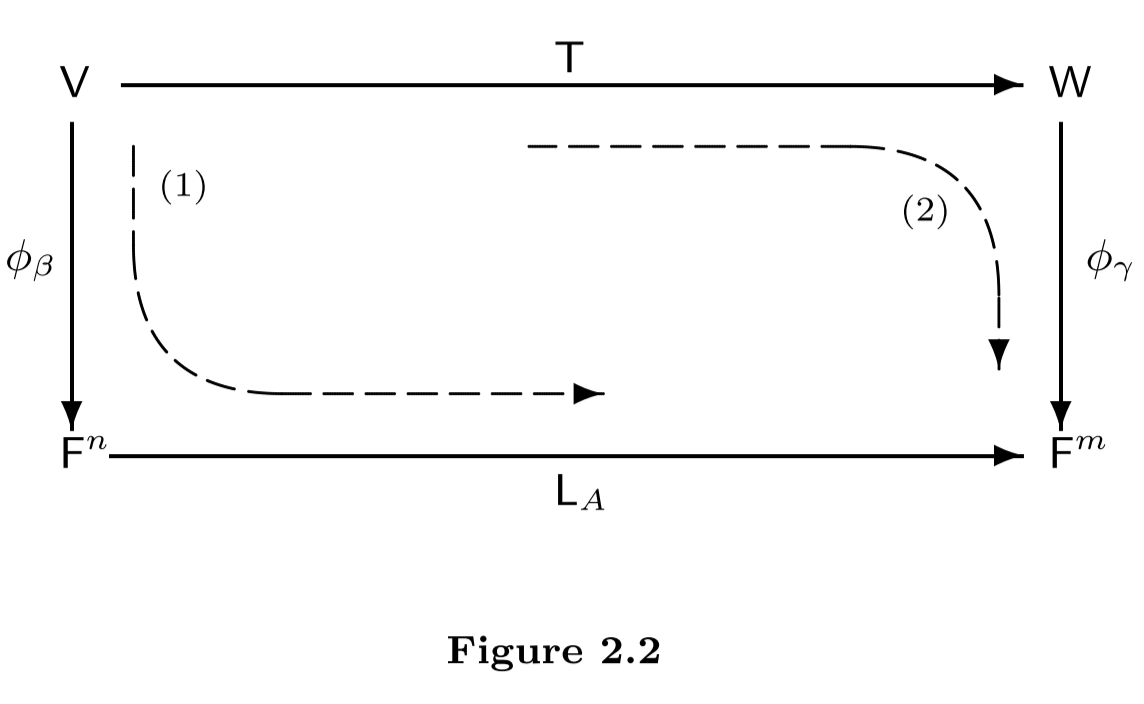
\includegraphics[width=16cm]{images/figure-2-2.png}

Let us first consider Figure 2.2.
Notice that there are two \emph{composites} of \LTRAN{}s that map \(V\) into \(F^m\):
\begin{enumerate}
\item[1.] Map \(V\) into \(F^n\) with \(\phi_{\beta}\) and follow this transformation with \(\LMTRAN_A\);
    this yields the composite \(\LMTRAN_A \phi_{\beta}\).
\item[2.] Map \(V\) into \(W\) with \(\T\) and follow it by \(\phi_{\gamma}\) to obtain the composite \(\phi_{\gamma} \T\).
\end{enumerate}

\begin{remark} \label{remark 2.4.6}
These two composites are depicted by the dashed arrows in the diagram.
By a simple reformulation of \THM{2.14}, we may conclude that for all \(v \in V\),
\begin{align*}
    \LMTRAN_A \phi_{\beta}(v)
    & = \LMTRAN_A (\phi_{\beta}(v)) & \text{by def of composition} \\
    & = \LMTRAN_A([v]_{\beta}) & \text{by def of \(\phi_{\beta}\)} \\
    & = A [v]_{\beta} & \text{by def of \(\LMTRAN_A\)} \\
    & = [\T]_{\beta}^{\gamma} [v]_{\beta} & \text{since \(A = [\T]_{\beta}^{\gamma}\)} \\
    & = [\T(v)]_{\gamma} & \text{by \THM{2.14}} \\
    & = \phi_{\gamma}(\T(v)) & \text{by def of \(\phi_{\gamma}\)} \\
    & = \phi_{\gamma} \T (v), & \text{by def of composition}
\end{align*}

Hence \(\LMTRAN_A \phi_{\beta} = \phi_{\gamma} \T\);
that is. the diagram ``commutes.'' (It seems that the terminology is from abstract algebra.)

Heuristically, this relationship indicates that after \(V\) and \(W\) are \emph{identified} with \(F^n\) and \(F^m\) via if \(\phi_{\beta}\) and \(\phi_{\gamma}\), respectively,
we may ``identify'' \(\T\) with \(\LMTRAN_A\).
\textbf{This diagram allows us to transfer operations on abstract vector spaces to ones on \(F^n\) and \(F^m\)}.
\end{remark}

\begin{example} \label{example 2.4.7}
Recall the \LTRAN{} \(\T : \mathcal{P}_3(\SET{R}) \to \mathcal{P}_2(\SET{R})\) defined in \EXAMPLE{2.2.4} (\(\T(f(x)) = f'(x)\)).
Let \(\beta\) and \(\gamma\) be the standard ordered bases for \(\mathcal{P}_3(\SET{R})\) and \(\mathcal{P}_2(\SET{R})\), respectively,
and let \(\phi_{\beta} : \mathcal{P}_3(\SET{R}) \to \SET{R}^4\) and \(\phi_{\gamma} : \mathcal{P}_2(\SET{R}) \to \SET{R}^3\) be the corresponding standard representations of \(\mathcal{P}_3(\SET{R})\) and \(\mathcal{P}_2(\SET{R})\).
If \(A = [\T]_{\beta}^{\gamma}\), then
\[
    A = \begin{pmatrix} 0 & 1 & 0 & 0 \\ 0 & 0 & 2 & 0 \\ 0 & 0 & 0 & 3 \end{pmatrix}
\]
Consider the polynomial \(p(x) = 2 + x - 3x^2 + 5x^3\).
We show that \(\LMTRAN_A \phi_{\beta} (p(x)) = \phi_{\gamma} \T (p(x))\).
Now
\[
    \LMTRAN_A \phi_{\beta} (p(x)) = [A]_{\beta}^{\gamma} [p(x)]_{\beta} 
    = \begin{pmatrix} 0 & 1 & 0 & 0 \\ 0 & 0 & 2 & 0 \\ 0 & 0 & 0 & 3 \end{pmatrix} \begin{pmatrix} 2 \\ 1 \\ -3 \\ 5 \end{pmatrix} = \begin{pmatrix} 1 \\ -6 \\ 15 \end{pmatrix}
\]
And since \(\T(p(x)) = p'(x) = 1 - 6x + 15x^2\), we have
\[
    \phi_{\gamma} \T (p(x)) = \phi_{\gamma} (1 - 6x + 15 x^2) = \begin{pmatrix} 1 \\ -6 \\ 15 \end{pmatrix}
\]
So \(\LMTRAN_A \phi_{\beta} (p(x)) = \phi_{\gamma} \T (p(x))\).
\end{example}
